%!TEX root = MemoireZelliges_simple.tex

\chapter{Bilan}
%======================================================================

\section{Comparaison entre les cinq zelliges étudiés}
%----------------------------------------------------------------------

\subsection{Description -- Texture}
%~~~~~~~~~~~~~~~~~~~~~~~~~~~~~~~~~~~~~~~~~~~~~~~~~~~~~~~~~~~~~~~~~~~~~~
On peut distinguer deux groupes distincts d'échantillons : d'une part, le zellige bleu, \frquote{pavé} servant à cerner le décor, et d'autre part les quatre zelliges vert, miel, noir et blanc, éléments du décor à proprement parler.

Ils se différencient tout d'abord par leur taille : le zellige bleu est beaucoup plus grand et plus épais (\SI{\sim4}{\cm} d'épaisseur pour le bleu, \SI{\sim2}{\cm} pour les autres) que les autres. Son substrat de céramique est également beaucoup plus rouge que les quatre zelliges plus petits, que l'on qualifierait plutôt d'ocre rose.

Les glaçures des zelliges vert, miel, noir et blanc présentent toutes des cassures franches et bien nettes. En revanche, on peut remarquer des coulures du mélange glaçurant sur le support de céramique du zellige bleu, réparties de manière homogène sur ses quatre faces.

On peut donc supposer que, contrairement au quatre autres, le zellige bleu n'a pas subit de découpe après l'application du mélange glaçurant et sa cuisson. La répartition homogène des coulures semble même indiquer que, lors de cette cuisson, le zellige était posé à plat, face glaçurée vers le haut.

L'étude de la texture de l'ensemble terre cuite-glaçure en lumière naturelle et \CL confirme cette ségrégation entre le zellige bleu et les quatre autres. En effet, le support de céramique du zellige bleu contient de grosses inclusions blanches et rouges observables à l'{\oe}il nu ainsi que quelques porosités de grande taille, réparties aléatoirement dans toute sa masse. À la loupe binoculaire, la terre cuite paraît très fine. En revanche, les terres cuites des quatre autres zelliges ne contiennent pas d'inclusions visibles à l'{\oe}il nu et sont assez peu poreuses. C'est l'observation à la loupe binoculaire qui y révèle la présence de nombreuses inclusions de couleurs variées (rouges, blanches, noires) et de granulométrie très fine (\SI{\sim0.15}{\mm}) réparties de manière homogène. De plus, la limite entre la glaçure et la terre cuite est très nette pour les quatre \frquote{petits} zelliges alors qu'elle est floue pour le bleu. On peut même parler de \frquote{fusion} des deux matériaux.

En \CL, on voit qu'aucune des glaçures ne luminesce mais que certaines (blanche, bleue) contiennent des cristaux de quartz (\ce{SiO2}) luminesçant en mauve.

La terre cuite du zellige bleu présente une luminescence à dominante mauve. Les autres présentent également une luminescence à dominante mauve mais avec de nombreuses luminescences ponctuelles rouges et bleues. De plus, dans le cas du zellige bleu, il faut noter, à l'interface terre cuite-glaçure, un liseré large qui luminesce en jaune et qui correspond à une bande de terre cuite plus clair en lumière naturelle. Pour les autres, on ne détecte pas ou peu de luminescences dans la zone d'interface.

L'observation au \MEB a permis de montrer que les luminescences aux interfaces ont pour origine des cristaux de dévitrification (des alumino-silicates mixtes de potassium, calcium et plomb).

Le très fort développement de la zone d'interface glaçure-terre cuite du zellige bleu peut laisser supposer des interactions fortes entre ces deux matériaux et donc l'application du mélange glaçurant sur une terre crue.

Dans les quatre autres zelliges, on trouve également des cristaux de dévitrification qui sont, selon ??? (199?), caractéristiques de l'application du mélange glaçurant sur une terre crue. Cependant les re-créations faites au laboratoire par Loïc~\bsc{Portelette} (1999, DESS) sont en contradiction avec ces résultats. De plus, le faible développement de l'interface semble indiquer peu d'interactions entre ces deux matériaux et donc, plutôt application du mélange glaçurant sur une terre cuite.

\subsection{Compositions élémentaires des glaçures}
%~~~~~~~~~~~~~~~~~~~~~~~~~~~~~~~~~~~~~~~~~~~~~~~~~~~~~~~~~~~~~~~~~~~~~~
\begin{figure}
  \begin{tikzpicture}
    \pgfplotstableread{\datadir/SpectroRX/PaM_BDX_SRX_gla.dat}
                      {\gladata}
    \pgfplotstablesort[sort key={bilan}]{\glasorted}{\gladata}

    \begin{axis}[
      bilan,
      ybar=0pt, bar width=5pt,
      title=Glaçures, title style={at={(0.33,0.85)}},
      ylabel=\PMO,
      x filter/.code={
        \pgfplotstablegetelem{\coordindex}{bilan}\of{\glasorted}
        \ifnumless{\pgfplotsretval}{99}{%
          %
        }{%
          \def\pgfmathresult{}
        }
      },
      xtick={0, ..., 10},
      xticklabels={
        \ce{SiO2},
        \ce{CaO},
        \ce{MgO},
        \ce{Na2O},
        \ce{K2O},
        \ce{Al2O3},
        \ce{PbO},
        \ce{SnO2},
        \ce{Fe2O3},
        \ce{CuO},
        \ce{MnO}
      },
    ]
      \addplot [fill=PaleGreen] 
         table [x expr=\coordindex, y=6528val, y error=6528err] 
         {\glasorted} ;
      \addlegendentry{Zellige vert}
      \addplot [fill=PowderBlue] 
         table [x expr=\coordindex, y=6529val, y error=6529err] 
         {\glasorted} ;
      \addlegendentry{Zellige bleu}
      \addplot [fill=Indigo] 
         table [x expr=\coordindex, y=6530val, y error=6530err] 
         {\glasorted} ;
      \addlegendentry{Zellige noir}
      \addplot [fill=Orange] 
         table [x expr=\coordindex, y=6531val, y error=6531err] 
         {\glasorted} ;
      \addlegendentry{Zellige miel}
      \addplot [fill=LightGoldenrod] 
         table [x expr=\coordindex, y=6532val, y error=6532err] 
         {\glasorted} ;
      \addlegendentry{Zellige blanc}
    \end{axis}

  \end{tikzpicture}
  \caption{\legendeAll 
           Compositions élémentaires des glaçures par \EDS. Toutes les glaçures sont plombifères. La glaçure verte est colorée par le \ce{Cu^2+}, la glaçure noire par le \ce{Mn^3+} et \ce{Fe^3+}, la glaçure miel par le \ce{Fe^3+}, la glaçure bleue est colorée par le \ce{Co^2+} et légèrement opacifiée à l'étain, la glaçure blanche est opacifiée à l'étain.}
  \label{plot:compo_gla}
\end{figure}

La \fref{plot:compo_gla} montre les compositions élémentaires de l'ensemble des glaçures. On peut constater qu'elles sont toutes plombifères. Elles ont donc été cuites en atmosphère oxydante car une cuisson réductrice aurait eu pour effet de noircir la glaçure. Les éléments chromogènes utilisés sont très classiques : le cobalt, sous la forme \ce{Co^2+} (comme le montre la \SAO), colore la glaçure bleue, associé à un peu d'étain pour adoucir la couleur et masquer la terre cuite rouge ; la coloration verte est due au cuivre dans l'état d'oxydation~II (montré par \SAO) ; le \ce{Mn^3+} associé au \ce{Fe^3+} donne sa coloration \frquote{orange foncé} à la glaçure noire ; la glaçure blanche est opacifiée par l'étain présent sous forme de cassitérite (\ce{SnO2}) et probablement par les fins cristaux de quartz non fondus présents à sa surface.

Il est intéressant de noter la plus faible teneur en plomb de la glaçure noire. Cela suppose qu'elle a été cuite à une température plus élevée que les autres.

La glaçure bleue ne contient quasiment pas d'oxyde d'aluminium, connu pour augmenter la viscosité du mélange glaçurant. Cela pourrait expliquer la position, à plat, de l'échantillon pendant la cuisson de ce mélange. En effet, si l'échantillon avait été placé debout \incise{comme c'est souvent le cas pour gagner de la place} le mélange glaçurant n'aurait probablement pas pu adhérer au support de céramique et aurait coulé.

\subsection{Compositions élémentaires des terres cuites}
%~~~~~~~~~~~~~~~~~~~~~~~~~~~~~~~~~~~~~~~~~~~~~~~~~~~~~~~~~~~~~~~~~~~~~~
\begin{figure}[htb]
  \begin{tikzpicture}
    \pgfplotstableread{\datadir/SpectroRX/PaM_BDX_SRX_tc.dat}%
                      {\tcdata}
    \pgfplotstablesort[sort key={bilan}]{\tcsorted}{\tcdata}

    \begin{axis}[
      bilan,
      ybar=0pt, bar width=5pt,
      title=Terres cuites, title style={at={(0.5,0.85)}},
      ylabel=\PMO,
      x filter/.code={
        \pgfplotstablegetelem{\coordindex}{bilan}\of{\tcsorted}
        \ifnumless{\pgfplotsretval}{99}{%
          %
        }{%
          \def\pgfmathresult{}
        }
      },
      xtick={0, ..., 8},
      xticklabels={
        \ce{SiO2},
        \ce{CaO},
        \ce{MgO},
        \ce{Na2O},
        \ce{K2O},
        \ce{Al2O3},
        \ce{Fe2O3},
        \ce{TiO2},
      },
    ]
      \addplot [fill=PaleGreen] 
         table [x expr=\coordindex, y=6528val, y error=6528err] 
         {\tcsorted} ;
      \addlegendentry{Zellige vert}
      \addplot [fill=PowderBlue] 
         table [x expr=\coordindex, y=6529val, y error=6529err] 
         {\tcsorted} ;
      \addlegendentry{Zellige bleu}
      \addplot [fill=Indigo] 
         table [x expr=\coordindex, y=6530val, y error=6530err] 
         {\tcsorted} ;
      \addlegendentry{Zellige noir}
      \addplot [fill=Orange] 
         table [x expr=\coordindex, y=6531val, y error=6531err] 
         {\tcsorted} ;
      \addlegendentry{Zellige miel}
      \addplot [fill=LightGoldenrod] 
         table [x expr=\coordindex, y=6532val, y error=6532err] 
         {\tcsorted} ;
      \addlegendentry{Zellige blanc}
    \end{axis}

  \end{tikzpicture}

  \caption{\legendeAll 
           Compositions élémentaires des terres cuites par 
           \EDS. Les terres 
           cuites sont très homogènes : elles sont de type calcique 
           et colorées par le fer en cuisson oxydante.}
  \label{plot:compo_tc}
\end{figure}

On peut constater sur la \fref{plot:compo_tc} que toutes les terres 
cuites sont de type calcique et que leur coloration rouge à ocre rose 
est due au fer présent sous la forme \ce{Fe^3+} en atmosphère de 
cuisson oxydante. C'est en fait le fer en excès, non piégé par les 
phases haute température dont le développement est favorisé par la 
présence de calcium.

L'homogénéité de composition des terres cuites peut apparaître comme 
contradictoire avec les différences de texture observées en lumière 
naturelle, \CL et \MEB[ie]. On peut émettre l'hypothèse que tous les 
échantillons ont été préparés à partir de la même matière première 
qui aurait subit une préparation différente selon l'emploi qui en est 
fait. Pour le zellige bleu, qui n'est pas un élément de décor mais une 
pièce utilisée pour le cerner, l'argile aurait subit une préparation 
assez sommaire. En revanche, l'argile utilisée pour fabriquer les 
éléments de décor aurait pu subir une décantation pour éliminer les 
inclusions les plus grosses (qui fragiliseraient le matériau lors de 
sa découpe) et, éventuellement, l'ajout d'un dégraissant minéral pour 
ajuster la plasticité du matériau aux besoins de l'artisan.

La teneur en fer est à peu près la même pour tous les échantillons, 
la différence de couleur entre le zellige bleu et les quatre autres 
pourrait s'expliquer par une atmosphère de cuisson légèrement plus 
oxydante pour le zellige bleu.

\subsection{Compositions \cristallo s des terres cuites}
%~~~~~~~~~~~~~~~~~~~~~~~~~~~~~~~~~~~~~~~~~~~~~~~~~~~~~~~~~~~~~~~~~~~~~~
Le \tref{tab:cristallo} présente les compositions \cristallo s des terres cuites des cinq échantillons. Toutes contiennent majoritairement du quartz, ainsi que de la calcite et diverses phases haute température (diopside, gehlénite, anorthite). On note également, pour les zelliges bleu, noir et miel, la présence d'albite.

Cette dernière disparaît vers \SI{850}{\degC}. Son association avec des phases haute température laisse penser que ces échantillons ont été cuits à une température de l'ordre de \SIrange[range-phrase=\ à\ ]{850}{900}{\degC}. Les zelliges vert et blanc auraient été cuits à une température légèrement plus élevée, de l'ordre de \SIrange[range-phrase=\ à\ ]{900}{950}{\degC}.


\begin{table}[htb]
  \sisetup{
    range-phrase = -
  }
  \centerfloat
  \noindent\begin{tabularx}{\textwidth}{X*{5}{M{1.7cm}}}
      ~ & \textbf{Zellige vert} & \textbf{Zellige bleu} & 
          \textbf{Zellige noir} & \textbf{Zellige miel} & 
          \textbf{Zellige blanc}
    \tabularnewline
    \otoprule
      \textbf{Quartz} (\ce{SiO2}) & 
      \blackstar & \blackstar & \blackstar & \blackstar & \blackstar
    \tabularnewline
    % \midrule
      \textbf{Calcite} (\ce{CaCO3}) & 
      \blackstar & \blackstar & \blackstar & \blackstar & \blackstar
    \tabularnewline
    % \midrule
      \textbf{Albite} &
       ~         & \bluestar  & \bluestar  & \bluestar  & ~
    \tabularnewline
    % \midrule
      \textbf{Diopside} &
      \blackstar & \blackstar & \blackstar & ~          & \blackstar
    \tabularnewline
    % \midrule
      \textbf{Gehlénite} &
      \blackstar & \blackstar & ~          & \blackstar & \blackstar
    \tabularnewline
    % \midrule
      \textbf{Anorthite} &
      \blackstar & ~          & ~          & \blackstar & \blackstar
    \tabularnewline
    % \midrule
      \textbf{Température de \mbox{cuisson} associée} (\si{\degC}) & 
      \numrange{900}{950} & \numrange{850}{900} & 
      \numrange{850}{900} & \numrange{850}{900} & 
      \numrange{900}{950}
    \tabularnewline
    \bottomrule
\end{tabularx}
\caption{\legendeAll 
         Compositions \cristallo s des terres cuites.}
\label{tab:cristallo}
\end{table}

\subsection{Étude de l'altération}
%~~~~~~~~~~~~~~~~~~~~~~~~~~~~~~~~~~~~~~~~~~~~~~~~~~~~~~~~~~~~~~~~~~~~~~
Nous n'avons détectées de figures d'altération chimique, que ce soit 
en lumière naturelle ou en \MEB[ie], dans aucun des cinq échantillons 
étudiés. En revanche, les cinq échantillons présentent une plus ou 
moins prononcée usure mécanique de surface.


\section{Proposition d'un protocole technologique}
%----------------------------------------------------------------------

L'ensemble de ces données nous a permis de proposer des hypothèses 
quant aux techniques de fabrications des zelliges. Il y aurait en fait 
deux techniques différentes selon l'utilisation de l'échantillon. Ces 
techniques sont résumées dans la \fref{fig:protocole}.

Dans le cas des pièces de grandes dimensions telles que le zellige 
bleu, utilisées pour cerner le décor, le potier procéderait au moulage 
d'un \frquote{pavé} parallélépipédique (de l'ordre de \SI{4}{\cm} 
d'épaisseur) à partir d'une argile préparé de manière assez sommaire. 
Il appliquerait ensuite sur ce support le mélange glaçurant et 
l'ensemble serait enfin soumis à une cuisson en atmosphère oxydante 
à une une température de l'ordre de
\SIrange[range-phrase=\ à\ ]{900}{950}{\degC}.

La même pâte argileuse subirait une préparation plus élaborée pour la 
mise en {\oe}uvre des éléments du décor, avec décantation et ajout de 
dégraissant minéral. De grand carreaux sont ensuite moulés et 
subissent peut-être une première cuisson oxydante à 
\SIrange[range-phrase=\ à\ ]{850}{900}{\degC}. Le mélange glaçurant 
est ensuite appliqué et l'ensemble est alors soumis à une deuxième (ou 
première) cuisson oxydante. Le maître-artisan peut ensuite procéder à 
la découpe des formes voulues et à leur assemblage.


\begin{figure}[p]
  \large
  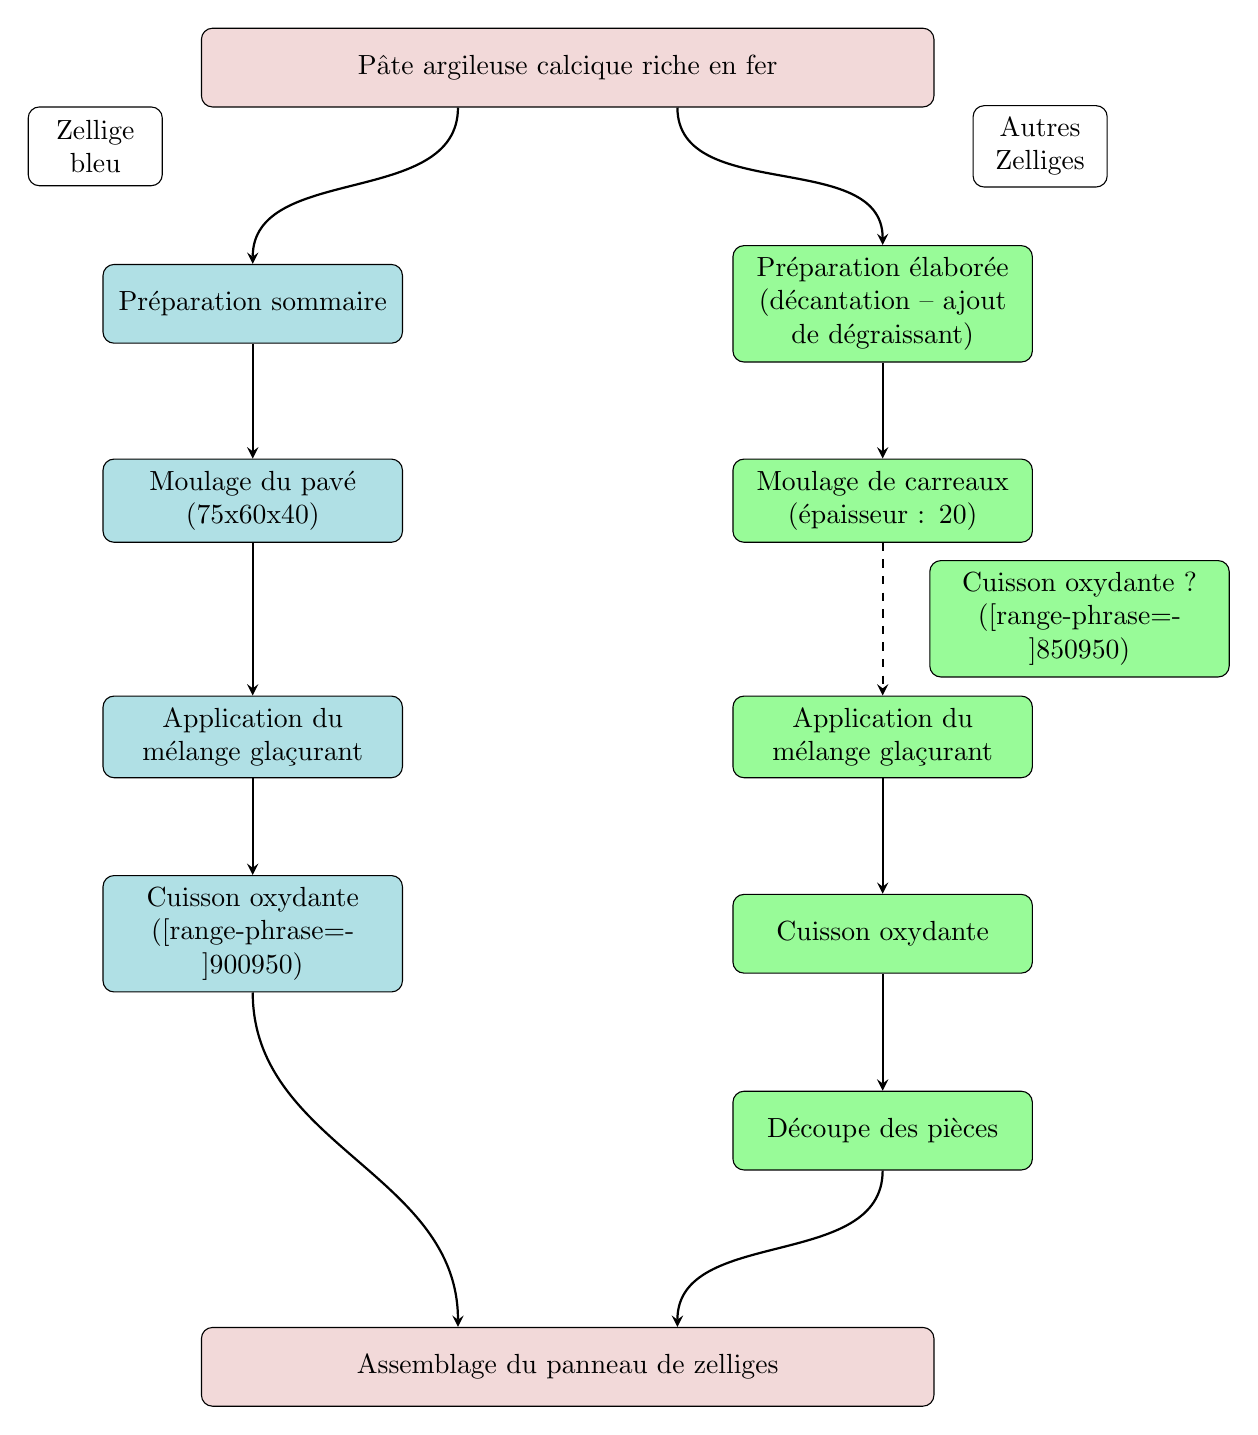
\begin{tikzpicture}[yscale=-1]
    \tikzset{
      every node/.style = {
        draw, rectangle, rounded corners, 
        font           = \smaller, 
        inner sep      = 1ex, 
        minimum height = 1cm, 
        minimum width  = 3.5cm,
        text width     = 3.5cm,
        align          = center
      },
      red/.style = {
        fill = gray!50!red!20, 
        minimum height = 1cm, 
        minimum width  = 9cm,
        text width     = 9cm,
      },
      blanc/.style = {
        minimum height = 1cm, 
        minimum width  = 1.4cm,
        text width     = 1.4cm,
      },
      bleu/.style = {
        fill = PowderBlue, 
        % fill = gray!50!blue!20, 
      },
      autre/.style = {
        fill = PaleGreen, 
        % fill = gray!50!green!20, 
      },
      flech/.style = {
        thick,
        ->,
        >=stealth,
      }
    }

    % \draw [help lines] (-8, 0) grid ( 8, 18) ;

    \node [red] (A) at ( 0.00, 0.00) 
          {Pâte argileuse calcique riche en fer} ;

    \node [blanc] (B0) at (-6.00, 1.00) 
          {Zellige bleu} ;
    \node [bleu]  (B1) at (-4.00,  3.00) 
          {Préparation sommaire} ;
    \node [bleu]  (B2) at (-4.00,  5.50) 
          {Moulage du pavé\\{\smaller(\SI{75x60x40}{\mm})}} ;
    \node [bleu]  (B4) at (-4.00,  8.50) 
          {Application du\\mélange glaçurant} ;
    \node [bleu]  (B5) at (-4.00, 11.00) 
          {Cuisson oxydante\\
           {\smaller(\SIrange[range-phrase=-]{900}{950}{\degC})}} ;

    \node [blanc] (C0) at ( 6.00,  1.00) 
          {Autres Zelliges} ;
    \node [autre] (C1) at ( 4.00,  3.00) 
          {Préparation élaborée\\
           {\smaller(décantation -- ajout de dégraissant)}} ;
    \node [autre] (C2) at ( 4.00,  5.50) 
          {Moulage de carreaux\\{\smaller(épaisseur : \SI{20}{\mm})}} ;
    \node [autre] (C3) at ( 6.50,  7.00) 
          {Cuisson oxydante ?\\
           {\smaller(\SIrange[range-phrase=-]{850}{950}{\degC})}} ;
    \node [autre] (C4) at ( 4.00,  8.50) 
          {Application du\\mélange glaçurant} ;
    \node [autre] (C5) at ( 4.00, 11.00) 
          {Cuisson oxydante} ;
    \node [autre] (C6) at ( 4.00, 13.50) 
          {Découpe des pièces} ;

    \node [red] (Z) at ( 0.00, 16.50) 
          {Assemblage du panneau de zelliges} ;

    \draw [flech] (A.200) to [out=90, in=-90] (B1.north) ;
    \draw [flech] (B1) -- (B2) ;
    \draw [flech] (B2) -- (B4) ;
    \draw [flech] (B4) -- (B5) ;
    \draw [flech] (B5.south) to [out=90, in=-90] (Z.160) ;

    \draw [flech] (A.-20) to [out=90, in=-90] (C1.north) ;
    \draw [flech] (C1) -- (C2) ;
    \draw [flech, dashed] (C2) -- (C4) ;
    \draw [flech] (C4) -- (C5) ;
    \draw [flech] (C5) -- (C6) ;
    \draw [flech] (C6.south) to [out=90, in=-90] (Z.20) ;
  \end{tikzpicture}
  \caption{Deux techniques de fabrications des zelliges à partir d'une 
           même argile calcique riche en fer. L'argile est préparée de 
           manière plus ou moins élaborée selon l'usage qu'il en est 
           fait.}
  \label{fig:protocole}
\end{figure}


\chapter{Perspectives}
%======================================================================

Notre étude a permis d'obtenir de nombreux indices sur les techniques 
de fabrication des zelliges de Meknès. Cependant, il reste encore des 
questions sans réponse (notamment, la question de l'application du 
mélange glaçurant sur terre crue ou cuite) et nos hypothèses doivent 
être vérifiées.

Il serait donc intéressant, pour valider ou infirmer notre proposition 
sur les techniques de fabrication des zelliges, de procéder à des 
essais de re-création en collaboration avec des céramistes et en 
utilisant des fours proches de ceux du \siecle{xvii} et des matières 
premières disponibles dans la région de Meknès.

Une étude comparative avec les échantillons de zelliges de Meknès 
datant du \siecle{xiv} étudiés cette année par Richard~\bsc{Cheret}, 
pourrait permettre d'obtenir des données sur l'évolution historique 
des techniques de fabrication de ce matériau. Il est nécessaire, pour 
cela, d'élargir l’échantillonnage à du matériel s'intercalant entre 
le \sclnum{xiv} et le \siecle{xvii} pour compléter cet 
\frquote{historique}.

Enfin, le deuxième volet de notre problématique de départ concernait 
l'altération des panneaux de zelliges qui se détachent en partie. Or, 
notre étude a montré que les zelliges eux-mêmes ne sont pas du tout 
altérés et ont bien résisté au temps. Il est donc nécessaire d'étudier 
les mortiers liant les pièces entre elles et permettant de maintenir 
le panneau au mur, puisque ce sont certainement eux qui sont 
responsables de ces dégradations.
